\chapter{The ABCD of Interest Rate Basis Spread}
\label{chap:abcd}

\section{Rationale for abcd modelling}

Given the problems and practical difficulties shown in \autoref{chap:bootstrapping} along with the inconsistency of \eqref{eq:no_arbitrage_forward_sc} from \autoref{chap:int_rate}, \cite{ametrano_ballabio_mazzocchi} thought to model the basis between an $x$ tenor simple forward and its corresponding overnight spanning forward as:

\begin{equation}
S_x(t) = F_x(t) - F_x^{ON}(t)\,,
\label{eq:S_x}
\end{equation}

where:

\begin{itemize}
    \item $t$ is measured with an arbitrary monotonically increasing day-count convention (usually $Actual/365(Fixed)$) between the corresponding date $d$ and the settlement date $d_0$ corresponding to $t_0=0$ (where $D(0)=1$);
    \item $x$ can be ON, 1M, 3M, 6M, 1Y;
    \item $F_x(t)$ is the forward rate which spans from time $t$ up to time $t+x$;
\end{itemize}

that empirically can be parameterized as:

\begin{equation}
S_x(t) = (A_x + B_x t)e^{-C_x t} + D_x\,.
\label{ABCD}
\end{equation}

The parameters have a particular meaning:
\begin{itemize}
    \item $A + D$ indicates the value of the basis in $t$ equals to 0;
    \item $D$ is the long run function value;
    \item $C$ indicates how quickly the function tends to D;
    \item $B$ indicates the additional time boost in order get the maximum value of function.
\end{itemize}

As it is clear, $A$ and $D$ have clear financial meaning while the other two cannot be so easily interpreted. Difficult in interpreting them, will lead to a modification in the following of the dissertation.

The basis is calibrated only using a subset of the instruments refereed to the $x$ modelled curve. The calibration of the basis is performed exploiting a best fit calibration algorithm such that is obtained:

\begin{equation}
F_x^{calib}(t) = S_x(t) + F_x^{ON}(t)\,.
\end{equation}

Subsequently, through an exact fit bootstrapping procedure, which exploits linear interpolation and therefore local scheme, the Rebonato correction factors are obtained:

\begin{equation}
K_x(t_i) = \frac{F_x^{mkt}(t_i)}{F_x^{calib}(t_i)}\,,
\label{direct-k}
\end{equation}

where $F_x^{mkt}(t_i)$ is the value of the contract quoted on the market and fixing at time $t_i$.
The corrector factors play a huge role, because allow to shape the information around an abcd basis while leaving the possibility to perfectly reproducing the observed curve and the embedded noise that belongs to the market.

\section{Relation between continuous and simple basis }

However, as already mentioned, in derivative world, the best practice is to model the quantity in continuous time, and it allows to model the instantaneous forward rate when retrieving the pseudo discount factor as in \eqref{eq:no_arbitrage_forward_sc_int} therefore it is introduced:

\begin{equation}
s_x(t) = f_x(t) - f_{ON}(t)\,,
\label{eq:s_x}
\end{equation}

where $f_x(t)$ is the instantaneous forward rate on the $x$ curve and $f_{ON}(t)$ is the instantaneous forward rate on the ON curve.

Egregious results are that the meaning of parameters is preserved and that exists an relation between continuous and simple basis:

\begin{equation}
1 + F_x(t) \tau_x(t) = e^{\int_t^{t+x} f_x(u) \mathrm{d}u}\,,
\end{equation} 

where:

\begin{itemize}
    \item $t+x$ is a shorthand for the time corresponding to the date $d_x=d+x$ which is a tenor $x$ later than the date $d$ corresponding to $t$ (according to all market and holiday conventions);
    \item $\tau_x(t, t+x)$ (in the following shortened as $\tau_x(t)$) is the year fraction between the dates $d$ and $d_x$ underlying the forward rate and measured according to its day-count convention $\tau_x$ (e.g., $Actual/360$ in the Euribor case).
\end{itemize}

Since $f_x(t) = s_x(t) + f_{ON}(t)$, we have:

\begin{equation}
\label{eq:forward_from_adj_disc}
\begin{split}
1 + F_x(t) \tau_x(t) &= e^{\int_t^{t+x} [s_x(u) + f_{ON}(u)] \mathrm{d}u}\\
&= [1 + F_x^{ON}(t) \tau_x(t)]e^{\int_t^{t+x} s_x(u) \mathrm{d}u}\,.
\end{split}
\end{equation}

Therefore:

\begin{equation}
e^{\int_t^{t+x} s_x(u) \mathrm{d}u} = \frac{1+ F_x(t) \tau_x(t)}{1+ F_x^{ON}(t) \tau_x(t)}\,. 
\end{equation}

Taking the logarithms and using a first-order approximation, we have:

\begin{equation}
\label{simple-vs-continuous}
\begin{split}
\int_t^{t+x} s_x(u) \mathrm{d}u &= \ln{\left[\frac{1+ F_x(t) \tau_x(t)}{1+ F_x^{ON}(t) \tau_x(t)}\right]}\\ 
&\approx F_x(t) \tau_x(t) - F_x^{ON}(t)\tau_x(t)\\
&= S_x(t) \tau_x(t)\,.
\end{split}
\end{equation}

Therefore it is possible to express the parameters of the simple basis $A$, $B$, $C$, $D$ as parameters of the continuous one $a$,$b$,$c$,$d$ as it follows:

\begin{equation}
\begin{split}
\int_t^{t+\tau_x} s_x(u) \mathrm{d}u &= \int_t^{t+\tau_x} \left[ (a_x + b_x u)e^{-c_x u} + d_x \right] \mathrm{d}u \\
                                     &= \left[\hat{A_x}(\tau_x) + \hat{B_x}(\tau_x) t\right] e^{-\hat{C}_x  t} + \hat{D_x}(\tau_x)
\end{split}
\end{equation}
with
\begin{equation}
\label{eq:integratedCoef}
\begin{split}
\hat{A_x}(\tau_x)&=-\left(\frac{a_x}{c_x}+ \frac{b_x}{c_x^{2}}+\frac{b_x}{c_x}\tau_x \right)e^{-c_x \tau_x}+\left(\frac{a_x}{c_x}+ \frac{b_x}{c_x^{2}}\right) \\
\hat{B_x}(\tau_x)&=\frac{b_x}{c_x}\left(1-e^{-c_x \tau_x}\right) \\
\hat{C_x}&=c_x \\
\hat{D_x}(\tau_x)&=d_x \tau_x\,.
\end{split}
\end{equation}

Substituting the above into equation~\ref{simple-vs-continuous}, we obtain
\begin{equation}
\left[\hat{A_x}(\tau_x) + \hat{B_x}(\tau_x) t\right] e^{-\hat{C}_x t} + \hat{D_x}(\tau_x) \approx S_x(t) \tau_x \,.
\end{equation}

Given that also with this new framework a best fit calibration was employed, in order to exact reprice the quote the following corrector factor has been locally bootstrapped according to:

\begin{equation}
\label{eq:bootstrapp_correcton_factors}
D_x^{adj}(t) = k_x(t) \cdot D_x^{calib}(t) = k_x(t) \cdot D_{ON}(t) \cdot e^{-\int_0^{t} s_x(u) \mathrm{d}u}
\end{equation}

in order to get:

\begin{equation}
F_x(t) = \frac{1}{\tau_x} \left[\frac{D^{adj}_x(t)}{D^{adj}_x(t+x)} - 1 \right]\,.
\end{equation}

The $k$ correction factors, differently from the basis, need to be bootstrapped in real time, because indicates how much it needs to be corrected the smooth basis in order to perform a perfect repricing of the market quotes.

Note: differently from basis, it is not possible to goes from continuous to simple correction factors.

\subsection{Generalized basis modelling}
In order to achieve better results the previous structure was applied but with incremental calibration, exploiting the generalized equation:

\begin{equation}
\begin{split}
S_{x,y}(t) &= F_x(t) - F_x^{y}(t)\\
s_{x,y}(t) &= f_x(t) - f_{y}(t)\,.
\end{split}
\end{equation}

At this point the authors, relying on the idea of modelling a basis as abcd, created two different framework one for the relative basis from incremental calibration and one for absolute basis with respect to the overnight rate in a not incremental calibration scheme.

Both the approaches led to extremely positive results, but the second allowed also to overcome the problematic shape of the retrieved 1M curve as it is possible to appreciate:

\begin{figure}[H]
\centering
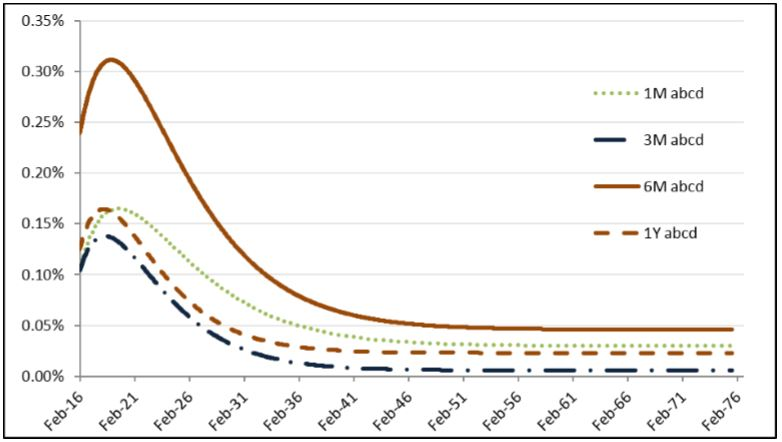
\includegraphics[scale=1]{abcd_basis_inc}
\caption{Basis from incremental calibration }
\label{fig:abcd_basis_inc}
\end{figure}

Unfortunately, it is not possible to shift from relative to absolute approach because difference of abcd with different exponential term does not lead to another abcd.
Anyway, it is worth to spot the vicinity of $c$ values for different tenors and for different type of calibration:

\begin{figure}[H]
\centering
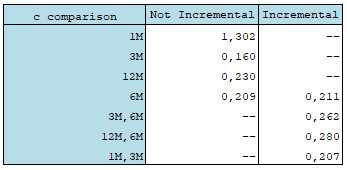
\includegraphics[scale=1]{abcd_c}
\caption{c parameters of the abcd basis}
\label{fig:abcd_c}
\end{figure}


\section{Contiguous basis times of maximum}

The authors noticed how the $t_{max}$ values were closed for each basis independently from the calibration choice:

\begin{figure}[H]
\centering
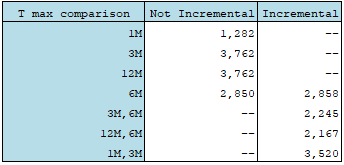
\includegraphics[scale=1]{abcd_t_max_comparison_inc_no_inc}
\caption{Abcd t max comparison}
\label{fig:abcd_t_max_comparison_inc_no_inc}
\end{figure}

robustly guessing a common value for it.
Moreover, they noticed how the simple basis peak anticipates the continuous one:

\begin{figure}[H]
\centering
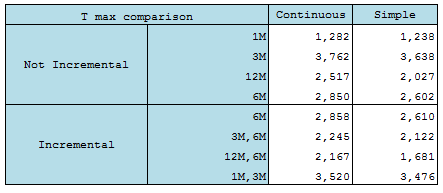
\includegraphics[scale=1]{abcd_t_max_comparison_simple_cont}
\caption{Abcd t max comparison: simple vs continuous}
\label{fig:abcd_t_max_comparison_simple_cont}
\end{figure}

which can be explained considering:

\begin{equation}
\int_t^{t+x} s_x(u) \mathrm{d}u = S_x(t) \tau_x(t)\,,
\end{equation}

the basis $ S_x(t)$ in $t$ incorporates the maximum value of $s_x(t_{max})$ anticipating de facto the max of s $s_x(t_{max})$.

It is possible to appreciate it with a graphical representation both not incremental

\begin{figure}[H]
\centering
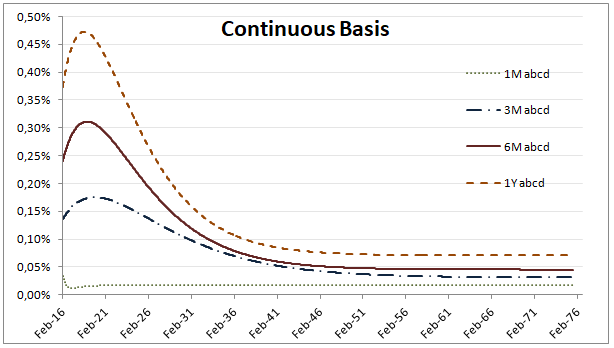
\includegraphics[scale=0.8]{abcd_basis_no_inc}
\caption{Basis from not incremental calibration }
\label{fig:abcd_basis_no_inc}
\end{figure}

and incremental

\begin{figure}[H]
\centering
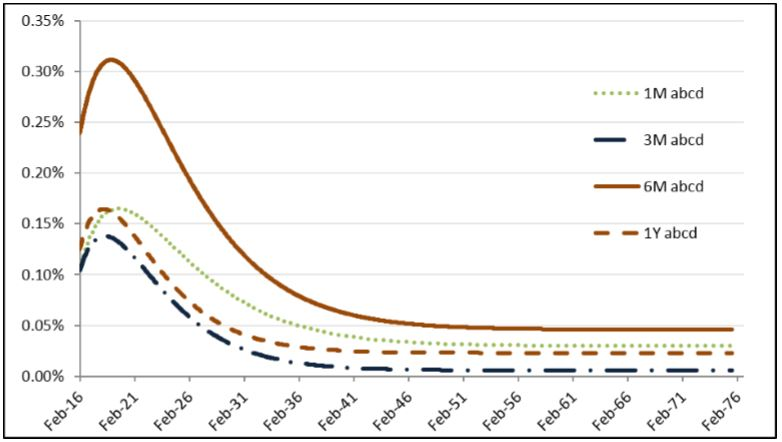
\includegraphics[scale=0.95]{abcd_basis_inc}
\caption{Basis from incremental calibration }
\end{figure}


In order to reconcile the absolute and relative basis, to evaluate the intuition of a financial common $t_{max}$ value and to look for parameters that embed a greater financial meaning, the abcd framework needs to be reviewed.